\documentclass[11pt,american,czech]{article}
\usepackage[T1]{fontenc}
\usepackage[utf8]{inputenc}
\usepackage[a4paper]{geometry}
\geometry{verbose,tmargin=1cm,bmargin=0.5cm,lmargin=1.5cm,rmargin=2cm,headheight=0.8cm,headsep=1cm,footskip=0.5cm}
\setcounter{secnumdepth}{3}
\usepackage{url}
\usepackage{amsmath}
\usepackage{amsthm}
\usepackage{amssymb}
\usepackage{graphicx}
\usepackage{setspace}

\usepackage{enumerate} %roman enumiration

\usepackage{threeparttable}
\usepackage{array}

\usepackage{multirow}
%\usepackage{booktabs} %for \cmidrule{a-b}
\usepackage{hhline}

%% C++ code
\usepackage{listings}
\usepackage{xcolor}
\lstset { %
	language=C++,
	backgroundcolor=\color{black!3}, % set backgroundcolor
	basicstyle=\footnotesize,% basic font setting
}

%% Use Times New Roman font for text and Belleek font for math
%% Please make sure that the 'esint' package is turned off in the
%% 'Math options' page.
\usepackage[varg]{txfonts}


%% Indent even the first paragraph in each section
\usepackage{indentfirst}

% completely avoid orphans (first lines of a new paragraph on the bottom of a page)
\clubpenalty=9500

% completely avoid widows (last lines of paragraph on a new page)
\widowpenalty=9500

% disable hyphenation of acronyms
\hyphenation{CDFA HARDI HiPPIES IKEM InterTrack MEGIDDO MIMD MPFA DICOM ASCLEPIOS MedInria}

%%---------------------------------------------------------------------

%% Print out all vectors in bold type instead of printing an arrow above them
%%\renewcommand{\vec}[1]{\boldsymbol{#1}}

% Replace standard \cite by the parenthetical variant \citep
%\renewcommand{\cite}{\citep}

\makeatother
\pagestyle{empty} %turns off page numbering

\usepackage{babel}
\begin{document}
\selectlanguage{czech}
\def\documentdate{24. dubna 2017}
\begin{flushright}
\textbf{	NUM2cv \\
	24. dubna 2017 \\
	Vladislav Belov}
\end{flushright}

\section{Rungeovy-Kuttovy metody}

Řešíme numericky Riccatiho rovnici~(\ref{uloha}) na intervalu $[0.25, 0.45]$ Rungeovými-Kuttovými metodami. Známe její analytické řešení: $u(t)=\big(\frac{1}{\sqrt{2}t}\tan{(\sqrt{2}(c-\frac{1}{t}))}-\frac{1}{2t}\big)e^{t}$, kde klademe $c=1$.

\begin{equation} \label{uloha}
	\begin{split}
		&\dot{u}(t)=t^{-4}e^{t}+u(t)+2e^{-t}u^{2}(t) = f\big(t, u\big), \\
		&u(0.25)=-31,1844.
	\end{split}
\end{equation}

\noindent
Označíme $\tau=$ \textit{integrationTimeStep}, $u_{0}=u(t_{0})$. Použijeme  metody:
\begin{enumerate}[I.]
	\item Runge-Kutta 1. řádu (Euler):
		\begin{equation*}
			\begin{split}
	&k_{1}(\tau)=\tau\cdot f\big(t_{0}, u_{0}\big), \\
	&u(t_0+\tau)=u(t) + k_{1}(\tau).
			\end{split}
		\end{equation*}
	\item Runge-Kutta 2. řádu: \label{RKII}
		\begin{equation*}
			\begin{split}
				&k_{1}(\tau)=\tau\cdot f\big(t_{0}, u_{0}\big), \\
				&k_{2}(\tau)=\tau\cdot f\big(t_{0}+\tau, u_{0}+k_{1}(\tau)\big), \\
				&u(t_0+\tau)=u(t) + \tfrac{1}{2}k_{1}(\tau)+\tfrac{1}{2}k_{2}(\tau).
			\end{split}
		\end{equation*}
	\item Runge–Kutta–Merson:
		\begin{equation*}
			\begin{split}
		&k_{1}(\tau) = \tau\cdot f(t_{0},u_{0}),\\
		&k_{2}(\tau) = \tau\cdot f \big( t_{0} + \tfrac13 \tau, u_{0} + \tfrac13 k_1 \big),\\
		&k_{3}(\tau) = \tau\cdot f \big( t_{0} + \tfrac13 \tau, u_{0} + \tfrac16 k_1 + \tfrac16 k_2 \big),\\
		&k_{4}(\tau) = \tau\cdot f \big( t_{0} + \tfrac12 \tau, u_{0} + \tfrac18 k_1 + \tfrac38 k_3 \big),\\
		&k_{5}(\tau) = \tau\cdot f \big( t_{0} + \tau, u_{0} + \tfrac12 k_1 - \tfrac32 k_3 + 2 k_4 \big),\\
		&u(t_{0}+\tau) = y_0 + \tfrac16 k_1 + \tfrac23 k_4 + \tfrac16 k_5.
			\end{split}
		\end{equation*}
\end{enumerate}

%\hrulefill
%\vspace{0.1cm} \\
\noindent
Soustředíme se na metodě ~(\ref{RKII}):

\begin{enumerate}[(a)]
	\item Průběh numerického řešení v porovnání s průběhem analytického ($timeStep = 10^{-2}$,  $integrationTimeStep = 10^{-3}$):
		\begin{figure}[ht!]
			\centering
			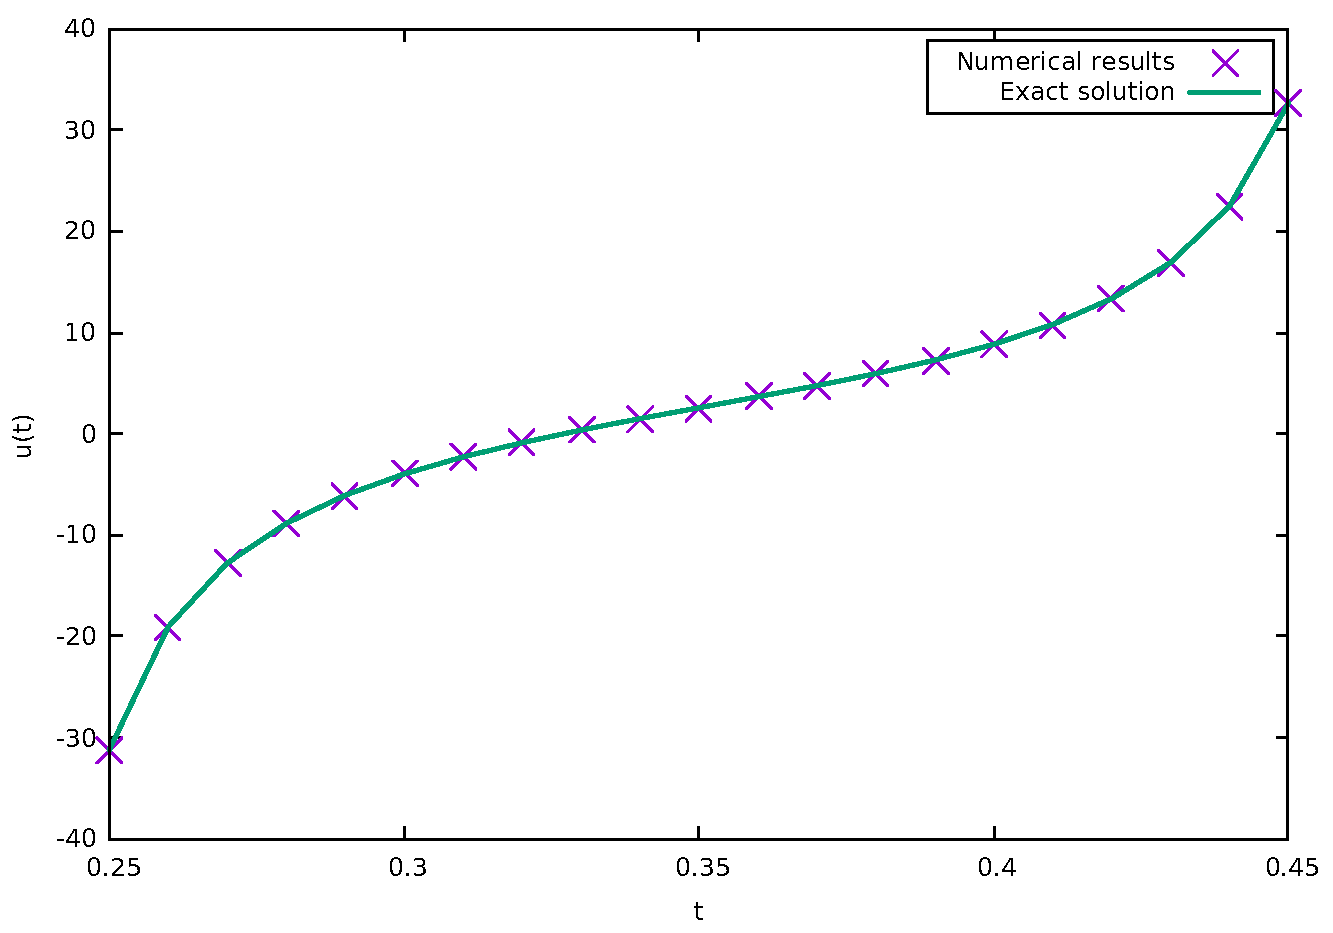
\includegraphics[height=8cm]{Figs/plot}
		\end{figure}
	\newpage
	\item Implementace:
		\begin{lstlisting}
		 
 template< typename Problem >
 class RungeKutta : public IntegratorBase
 {
  public:

   RungeKutta( Problem& problem )
   {
	this->k1 = new double[ problem.getDegreesOfFreedom() ];
	this->k2 = new double[ problem.getDegreesOfFreedom() ];
	this->aux = new double[ problem.getDegreesOfFreedom() ];
   }

   bool solve( Problem& problem,
		double* u )
   {
	const int dofs = problem.getDegreesOfFreedom();
	double tau = std::min( this->integrationTimeStep, this->stopTime - this->time );
	long int iteration( 0 );
	while( this->time < this->stopTime )
	{
	  /****
	  * Compute k1
	  */
	  problem.getRightHandSide( this->time, u, k1 );

	  /****
	  * Compute k2
	  */
	  for( int i = 0; i < dofs; i++ )
	    aux[ i ] = u[ i ] + tau * k1[ i ];
	  problem.getRightHandSide( this->time + tau, aux, k2 );

	  /****/
	  for( int i = 0; i < dofs; i++ )
	    u[ i ] += ( tau / 2.0 ) * ( k1[ i ] + k2[ i ] );
	  this->time += tau;
	  iteration++;
	  if( iteration > 100000 )
	  {
	    std::cerr << "The solver has reached the maximum number of iteratoins. " 
	    		<< std::endl;
	    return false;
	  }
	  tau = std::min( tau, this->stopTime - this->time );
	  std::cout << "ITER: " << iteration << " \t tau = " << tau 
	  		<< " \t time= " << time << "         \r " << std::flush;  
	}
	std::cout << std::endl;
	return true;
   }

   ~RungeKutta()
   {
	delete[] k1;
	delete[] k2;
	delete[] aux;
   }

  protected:

   double *k1, *k2, *aux;

 };
		\end{lstlisting}

\end{enumerate}

\newpage

\section{$L^{1}$, $L^{2}$, $L^{\infty}$ - normy, EOC (experimental orders of convergence)}

Označíme $\tau = integrationTimeStep$, $\Delta t = timeStep$ (pro výpočet norem položíme $\tau = \Delta t$), $\bar{u}_{\tau}$ - numerické řešení spočítané s integračním krokem $\tau$, $u$ - analytické řešení, $K$ - počet bodů v rozdělení intervalu $[a, b]$ ($a=0.25$, $b=0.45$, $K = \tfrac{b-a}{\Delta t}$). Potom lze spočítat normy takto:

\begin{equation*}
	\begin{split}
		&\rVert\bar{u}_{\tau}-u\lVert_{L^{1}} = \sum_{j=0}^{K}\lvert\bar{u}_{\tau}(a+j\Delta t)-u(a+j\Delta t)\rvert\cdot\Delta t \\
		&\rVert\bar{u}_{\tau}-u\lVert_{L^{2}} = \Big(\sum_{j=0}^{K}\lvert\bar{u}_{\tau}(a+j\Delta t)-u(a+j\Delta t)\rvert^{2}\cdot\Delta t\Big)^{\frac{1}{2}} \\
		&\rVert\bar{u}_{\tau}-u\lVert_{L^{\infty}} = \max_{j=0,1,\cdots,K}\  \lvert\bar{u}_{\tau}(a+j\Delta t)-u(a+j\Delta t)\rvert 
	\end{split}
\end{equation*}

\noindent
Chyba (err.) metody se spočte jako $E_{\tau} = \rVert\bar{u}_{\tau}-u\lVert_{L}$ a experimentální řád konvergence EOC($E_{\tau_{1}}$, $E_{\tau_{2}}$) $= {\log_{2}{\tfrac{E_{\tau_{1}}}{E_{\tau_{2}}}}}\big/{\log_{2}{\tfrac{\tau_{1}}{\tau_{2}}}}$.
\begin{table}[!htb]
	\centering\shorthandoff{-}
	\renewcommand{\arraystretch}{1.2}
	\begin{tabular}{ |c||c|c|c|c|c|c| }
	  \hline
%	 \multirow{2}{*}{Defenders} & LB & Lucas Radebe \\
%	  & DC & Michael Duburry \\

	\multirow{2}{*}{$\tau$} & \multicolumn{2}{c|}{$L^{1}$} & \multicolumn{2}{c|}{$L^{2}$} & \multicolumn{2}{c|}{$L^{\infty}$} \\ \hhline{~------}
	& err. &  EOC & err. & EOC & err. & EOC \\
	  \hline \hline
	$2\cdot10^{-3}$ & $3.27189\cdot10^{-1}$ & $\times$ & $1.18346$ & $\times$ & $11.7741$ & $\times$  \\ \hline 
	$1\cdot10^{-3}$ & $1.49554\cdot10^{-1}$ & $1.12946$ & $5.22467\cdot10^{-1}$ & $1.1796$ & $5.20364$ & $1.17802$ \\ \hline
	$5\cdot10^{-4}$ & $7.17241\cdot10^{-2}$ & $1.06013$ & $2.46576\cdot10^{-1}$ & $1.0833$ & $2.45653$ & $1.0829$  \\ \hline
	$2.5\cdot10^{-4}$ & $3.51473\cdot10^{-2}$ & $1.02904$ & $1.19901\cdot10^{-1}$ & $1.04019$ & $1.19462$ & $1.25532$  \\ \hline
	$1.25\cdot10^{-4}$ & $1.74006\cdot10^{-2}$ & $1.01428$ & $5.91353\cdot10^{-2}$ & $1.01975$ & $5.89204\cdot10^{-1}$ & $0.80446$  \\ \hline
	$6.25\cdot10^{-5}$ & $8.65769\cdot10^{-3}$ & $1.00708$ & $2.93677\cdot10^{-2}$ & $1.00979$ & $2.92613\cdot10^{-1}$ & $1.00977$  \\ \hline
	\end{tabular}
	\caption{Eulerova metoda}
	\vspace{0.75cm}
	\begin{tabular}{ |c||c|c|c|c|c|c| }
	  \hline
	\multirow{2}{*}{$\tau$} & \multicolumn{2}{c|}{$L^{1}$} & \multicolumn{2}{c|}{$L^{2}$} & \multicolumn{2}{c|}{$L^{\infty}$} \\ \hhline{~------}
	& err. &  EOC & err. & EOC & err. & EOC \\
	  \hline \hline
	$2\cdot10^{-3}$ & $6.09946\cdot10^{-3}$ & $\times$ & $2.39973\cdot10^{-2}$ & $\times$ & $2.70752\cdot10^{-1}$ & $\times$  \\ \hline 
	$1\cdot10^{-3}$ & $1.48308\cdot10^{-3}$ & $2.04009$ & $5.79622\cdot10^{-3}$ & $2.04969$ & $6.82516\cdot10^{-2}$ & $1.98804$ \\ \hline
	$5\cdot10^{-4}$ & $3.64603\cdot10^{-4}$ & $2.0242$ & $1.41923\cdot10^{-3}$ & $2.03$ & $1.70738\cdot10^{-2}$ & $1.99908$  \\ \hline
	$2.5\cdot10^{-4}$ & $9.03309\cdot10^{-5}$ & $2.01303$ & $3.50848\cdot10^{-4}$ & $2.01619$ & $4.26622\cdot10^{-3}$ & $2.00075$  \\ \hline
	$1.25\cdot10^{-4}$ & $2.24775\cdot10^{-5}$ & $2.00674$ & $8.72043\cdot10^{-5}$ & $2.00837$ & $1.06606\cdot10^{-3}$ & $2.00067$  \\ \hline
	$6.25\cdot10^{-5}$ & $5.60607\cdot10^{-6}$ & $2.00342$ & $2.17368\cdot10^{-5}$ & $2.00426$ & $2.66439\cdot10^{-4}$ & $2.00041$  \\ \hline
	\end{tabular}
	\caption{Rungeova-Kuttova metoda 2. řádu}
	\vspace{0.75cm}
	\begin{tabular}{ |c||c|c|c|c|c|c| }
	  \hline
%	 \multirow{2}{*}{Defenders} & LB & Lucas Radebe \\
%	  & DC & Michael Duburry \\

	\multirow{2}{*}{$\tau$} & \multicolumn{2}{c|}{$L^{1}$} & \multicolumn{2}{c|}{$L^{2}$} & \multicolumn{2}{c|}{$L^{\infty}$} \\ \hhline{~------}
	& err. &  EOC & err. & EOC & err. & EOC \\
	  \hline \hline
	$2\cdot10^{-3}$ & $3.2243\cdot10^{-6}$ & $\times$ & $1.21815\cdot10^{-5}$ & $\times$ & $1.35241\cdot10^{-4}$ & $\times$  \\ \hline 
	$1\cdot10^{-3}$ & $1.94926\cdot10^{-7}$ & $4.04799$ & $7.27902\cdot10^{-7}$ & $4.0648$ & $8.3966\cdot10^{-6}$ & $4.00958$ \\ \hline
	$5\cdot10^{-4}$ & $1.19626\cdot10^{-8}$ & $4.02632$ & $4.44086\cdot10^{-8}$ & $4.03483$ & $5.22349\cdot10^{-7}$ & $4.00672$  \\ \hline
	$2.5\cdot10^{-4}$ & $7.40577\cdot10^{-10}$ & $4.01374$ & $2.74112\cdot10^{-9}$ & $4.018$ & $3.25602\cdot10^{-8}$ & $4.00383$  \\ \hline
	$1.25\cdot10^{-4}$ & $4.60616\cdot10^{-11}$ & $4.00701$ & $1.70236\cdot10^{-10}$ & $4.00916$ & $2.0321\cdot10^{-9}$ & $4.00207$  \\ \hline
	$6.25\cdot10^{-5}$ & $6.64083\cdot10^{-12}$ & $2.79413$ & $2.64732\cdot10^{-11}$ & $2.68493$ & $3.09228\cdot10^{-10}$ & $2.71623$  \\ \hline
	\end{tabular}
	\caption{Rungeova-Kuttova-Mersonova metoda (bez adaptivity)}
\end{table}


\end{document}
